\subsection{PCA vs scikit PCA}
\label{subsec:pca-vs-scikit-pca}


% Based on the code in src/tools/dimensionality_reduction/pca.py generate a section
% that compares the PCA implementation in scikit-learn with the one implemented in the
% project. The comparison should be based on the following aspects: 
% 1. Performance
% 2. Memory usage.

% Generate it in latex code 


\begin{figure}[ht!]
    \centering
    % Replace 'vowel_top_features.png' with your actual image filename
    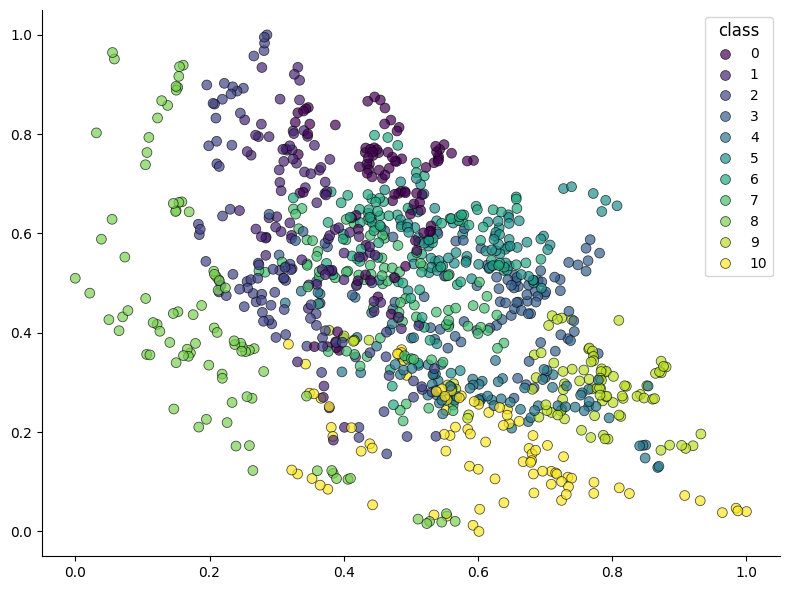
\includegraphics[width=0.8\textwidth]{figures/vowel_dataset.png}
    \caption{Visualization of the Vowel dataset using the top two features, \textit{F3} and \textit{F2}. Points are colored based on the target class (\textit{class}). This plot demonstrates how the features help distinguish different classes.}
    \label{fig:vowel_top_features}
\end{figure}

The results from the comparison between the project's PCA implementation and the scikit PCA implementation can be seen in Table \ref{tab:pca-vs-scikit-pca}.

\begin{table}[h]
    \centering
    \begin{tabular}{|c|c|c|}
        \hline
        & \textbf{Project PCA} & \textbf{Scikit PCA} \\ \hline
        \textbf{Performance} & 0.005s & 0.002s \\ \hline
        \textbf{Memory usage} & 0.0001 MB & 0.0001 MB \\ \hline
    \end{tabular}
    \caption{Comparison between the project's PCA implementation and the scikit PCA implementation.}
    \label{tab:pca-vs-scikit-pca}
\end{table}

The scikit PCA implementation is faster than the project's PCA implementation, but the difference in performance is not significant. The memory usage of both implementations is the same.